\documentclass{article}
\usepackage{pst-eucl}
\usepackage{changepage, amsmath, amssymb, pgfplots, tikz}
\usetikzlibrary{fit,positioning}
\usepgfplotslibrary{groupplots}
\usepackage[utf8]{inputenc}
\psset{PointName=none,PointSymbol=none}
\usetikzlibrary{arrows.meta}	
\usetikzlibrary{calc,patterns,angles,quotes}
\pgfplotsset{compat=1.16}
\usetikzlibrary{arrows.meta}
\usepackage{fullpage}
\usepackage{xparse,array}
\usetikzlibrary{circuits.ee.IEC}
\usepackage{ulem}
\usepackage{mathtools}
\usepackage{tikz}
\usetikzlibrary{tikzmark,calc}
\usepackage{geometry,graphicx}				% Paquetes adicionales.
\usepackage{subcaption,array}
\usepackage{multicol,multirow}
\usepackage{mathtools}
\usepackage{circuitikz,siunitx}
\usepackage{xcolor}
\usetikzlibrary{circuits.ee.IEC}
\usepackage[colorlinks=true, urlcolor=mypurple, linkcolor=mypurple]{hyperref}
\usetikzlibrary{trees}
\usepackage[dvipsnames]{xcolor}
\usepackage{darkmode}
\enabledarkmode
\usepackage{framed} % or, "mdframed"
\usepackage{fancyhdr}
\usepackage{fontawesome}
\pagestyle{fancy}
\usepackage[framed]{ntheorem}
\usepackage{lmodern}
\usepackage{tabularx}
\usepackage{microtype}
\setlength{\columnsep}{1.5cm}
\setlength{\columnseprule}{0.4pt}
\usepackage{multicol}
\usetikzlibrary{arrows, shapes.gates.logic.US, calc}
\usetikzlibrary{calc,arrows.meta}
\usepackage[most]{tcolorbox}
\definecolor{p1}{HTML}{caf0f8}
\definecolor{p2}{HTML}{ade8f4}
\definecolor{p3}{HTML}{90e0ef}
\definecolor{p4}{HTML}{48cae4}
\definecolor{p5}{HTML}{00b4d8}
\definecolor{p6}{HTML}{0096c7}
\definecolor{p7}{HTML}{0077b6}
\definecolor{p8}{HTML}{023e8a}
\definecolor{p9}{HTML}{03045e}
\usepackage{multicol}
\usetikzlibrary {arrows.meta,graphs,shapes.misc}
\usetikzlibrary {positioning}
\usepackage{colortbl}
\colorlet{xcol}{blue!60!black}
\usepackage{capt-of}
\definecolor{myred}{HTML}{f44336}
\definecolor{mypink}{HTML}{e81e63}
\definecolor{mypurple}{HTML}{9c27b0}
\definecolor{mydeeppurple}{HTML}{673ab7}
\definecolor{myindigo}{HTML}{3f51b5}
\definecolor{myblue}{HTML}{2196f3}
\definecolor{mylightblue}{HTML}{03a9f4}
\definecolor{mycyan}{HTML}{00bcd4}
\definecolor{myteal}{HTML}{009688}
\definecolor{mygreen}{HTML}{4caf50}
\definecolor{mylightgreen}{HTML}{8bc34a}
\definecolor{mylime}{HTML}{cddc39}
\definecolor{myyellow}{HTML}{ffeb3b}
\definecolor{myamber}{HTML}{ffc107}
\definecolor{myorange}{HTML}{ff9800}
\definecolor{mydeeporange}{HTML}{ff5722}
\definecolor{mybrown}{HTML}{795548}
\definecolor{mygray}{HTML}{9e9e9e}
\definecolor{mybluegray}{HTML}{607d8b}
\definecolor{pag}{HTML}{293133}
\usepackage[labelformat=empty]{caption}
\usepackage{mdframed}
\newtcolorbox{qq}[2][]{%
	boxrule=0.75pt,
	sharp corners,  % Square edges
	colframe=white,  % Set the color of the outline
	colback=pag,  % Set the color of the fill
	coltext=white,
	#1,
}
\usepackage[framed]{ntheorem}
\newframedtheorem{frm-thm}{Theorem}

%portrail

\title{Análisis Matemático I}
\date{\today}
\author{Alejandro Ceccheto}
\begin{document}
	\maketitle
	\pagebreak
	
	\section{Teoría}


\vspace{0.5cm}
\begin{center}
	\begin{framed}
		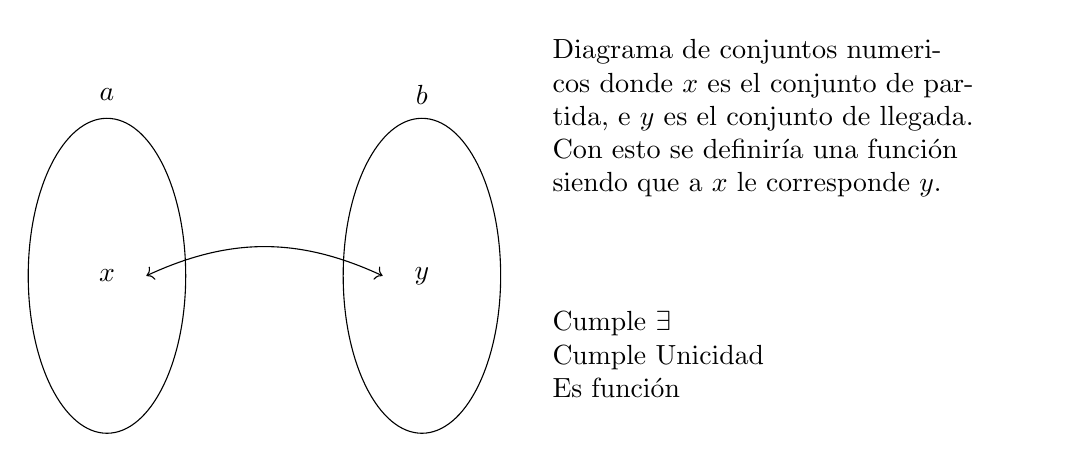
\begin{tikzpicture}
		\node at (0,2.3) {$a$};
		\node at (4,2.3) {$b$};
		\draw (0,0) ellipse [x radius = 1cm, y radius = 2cm];
		\draw (4,0) ellipse [x radius = 1cm, y radius = 2cm];
		\draw (0,0) node {$x$};
		\draw (4,0) node {$y$};
		\draw[<->] (0.5,0) to [bend left=25] (3.5,0);
		\draw ;
		\node at (4.5,2) [right=1cm,text width=6cm,rounded corners,inner sep=1ex,]
		{ Diagrama de conjuntos numericos donde $x$ es el conjunto de partida, e $y$ es el conjunto de llegada. \linebreak
			Con esto se definiría una función siendo que a $x$ le corresponde $y$.
		};
		\node  at (4.5,-1)[right=1cm,text width=6cm,rounded corners,inner sep=1ex,]{Cumple $\exists$ \\
		          Cumple Unicidad \\
		          Es función};
	\end{tikzpicture}
	\end{framed}
\end{center}
	

\begin{center}
	\begin{framed}
		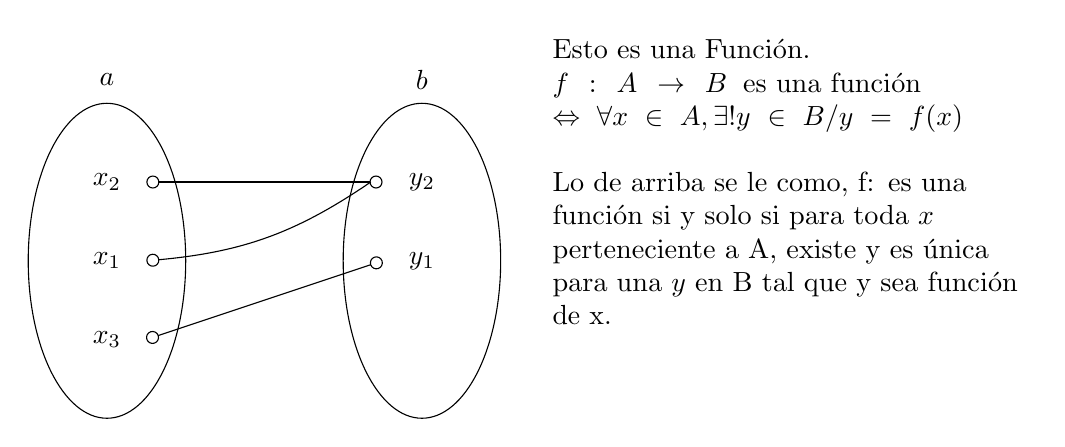
\begin{tikzpicture}
			\draw (0,0) ellipse [x radius = 1cm, y radius = 2cm];
			\draw (4,0) ellipse [x radius = 1cm, y radius = 2cm];
			\draw (0,0) node {$x_1$};
			\draw (0,1) node {$x_2$};
			\draw (0,-1) node {$x_3$};
			\draw (4,0) node {$y_1$};
			\draw (4,1) node {$y_2$};
			
			
			\draw[o-o] (0.5,-1) to (3.5,0);
			\draw[o-] (0.5,0)  to [bend right=15]  (3.35,1);
			\draw[o-o] (0.5,1)  to (3.5,1);
			\node at (4.5,1) [right=1cm,text width=6cm,rounded corners,inner sep=1ex,]
			{Esto es una Función. \linebreak
			$f : A \rightarrow B \hspace{0.2cm} $es una función$ \hspace{0.2cm} $\linebreak$ \Leftrightarrow   \forall x \in A, \exists! y \in B / y = f(x) $ \linebreak
			
			
			Lo de arriba se le como, f: es una función si y solo si para toda $x$ perteneciente a A, existe y es única para una $y$ en B tal que y sea función de x.};
			\node at (0,2.3) {$a$};
			\node at (4,2.3) {$b$};
		\end{tikzpicture}
	\end{framed}
\end{center}

	
\begin{center}
	\begin{framed}
		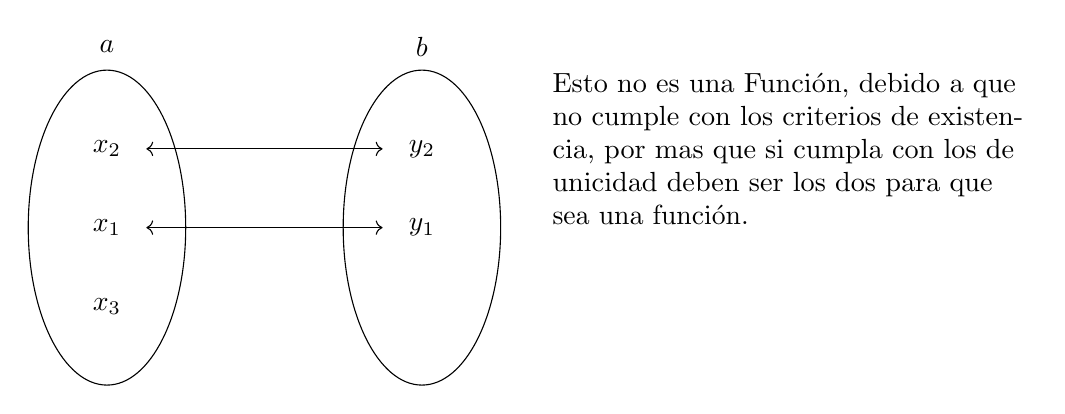
\begin{tikzpicture}
			\node at (0,2.3) {$a$};
			\node at (4,2.3) {$b$};
			\draw (0,0) ellipse [x radius = 1cm, y radius = 2cm];
			\draw (4,0) ellipse [x radius = 1cm, y radius = 2cm];
			\draw (0,0) node {$x_1$};
			\draw (0,1) node {$x_2$};
			\draw (0,-1)node {$x_3$};
			\draw (4,0) node {$y_1$};
			\draw (4,1) node {$y_2$};
			
			\draw[<->] (0.5,1) to (3.5,1);
			\draw[<->] (0.5,0) to  (3.5,0);
			
			\node at (4.5,1) [right=1cm,text width=6cm,rounded corners,inner sep=1ex,]
			{Esto no es una Función, debido a que no cumple con los criterios de existencia, por mas que si cumpla con los de unicidad deben ser los dos para que sea una función.};
		\end{tikzpicture}
	\end{framed}
\end{center}	

\section{Ejemplo.}
\vspace{0.3cm}
Como ejemplo se utilizo una función raíz cuadrada de lo mas conocida, generalmente es utilizada para explicar el tema.

	\begin{framed}
		\begin{equation*}
			\sqrt{x-1}
		\end{equation*}
		\begin{center}
			\begin{tikzpicture}[scale=0.9]
				\begin{axis}[axis lines=center, minor tick num=3]
					\addplot[samples=80, smooth, thick, domain=0:10]
					{sqrt(x-1)};
					
				\end{axis}
			\end{tikzpicture}
		\end{center}
	\end{framed}
	
	\subsubsection{Desarrollo.}
	
	
	$h: D_h \rightarrow \mathbb{R} / h(x) = \sqrt{x-1}$
	
	\begin{center}
		\begin{equation*}
			x-1 \geq 0 
		\end{equation*}
		\begin{equation*}
			x \geq 1
		\end{equation*}
		\begin{equation*}
			D_h = [1;+\infty) \hspace{0.2cm} \neq \hspace{0.2cm} \mathbb{R}^+ - \left\{1\right\}
		\end{equation*}
		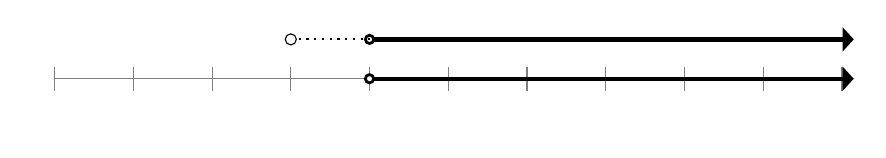
\begin{tikzpicture}[
			line/.style = {draw, ultra thick, shorten <=-2pt},
			La/.style = {line, shorten >=-2pt,
				{Circle[length=4pt, line width=1pt]}-{Circle[length=4pt,line width=1pt, fill=white]}},
			Lb/.style = {line, shorten >=-2pt,
				{Circle[length=4pt, line width=1pt, fill=white]}-{Circle[length=4pt, line width=1pt]}},
			Lc/.style = {line,
				{Circle[length=4pt, line width=1pt, fill=white]}-{Triangle[length=4pt, line width=1pt]}},
			Lq/.style = {line, shorten >=-2pt,
				{Circle[length=4pt, line width=1pt, fill=white]}-{Circle[length=4pt,line width=1pt, fill=white]}},
			Ld/.style = {line, shorten >=-2pt,
				{Circle[length=4pt, line width=1pt]}-{Circle[length=4pt, line width=1pt]}},
			Ldo/.style = {dotted, shorten >=-2pt,
				{Circle[length=4pt, line width=1pt]}-{Circle[length=4pt,line width=1pt, fill=white]}},	
			]
		
					\draw[gray] (-3,0) -- (7,0);    % <---
					\foreach \i in {-3,-2,...,7} % numbers on line
					\draw[gray] (\i,0.15) -- ++ (0,-0.3)    % <---
					node[below,text=white] {$\i$}; % tick and their labels
					
					\draw[Lc] (1,0) to (7.15,0) ;
					\draw[Lc] (1,0.5) to (7.15,0.5);
					\draw[dotted, thick] (0,0.5) to (1,0.5);
					\draw[fill=white] (0,0.5) circle[radius = 2pt];
					
		\end{tikzpicture}
	\end{center}
	
\end{document}